In this research, we propose a novel interoperable fuzzing architecture that is
environment- and platform-independent. Our Killerbeez solution disseminates
into four major components of drivers, mutators, instrumentation, a seed
selection algorithm and corpus minimization. A distributed computing model is
achieved by using multiple worker nodes fuzzing in parallel which obtain work
from, and return results to, a central server.

While there are some novel improvements in Killerbeez, it is important to
remember that the primary benefit is getting so many existing tools to work
together.  Each tool which was pulled in was the best in class on its own, but
when combined the value is more than just the sum of all its parts.

\subsection{Driver} \label{Driver}
Driver modules use the mutator module which is passed in to mutate an input,
the instrumentation module to trace the target's execution, and are responsible
for getting the input data into the program.  A simple example would be a
file-based driver, which will create a file containing the mutated input and
use the instrumentation module to launch the application in a way that it will
read this file.  This is typically accomplished by passing a filename in on the
command line.  For targets which do not have any way to specify the input file
on the command line, a custom driver would be required to use keyboard
shortcuts, mouse input, or some other method of getting the file into the
program.

The following drivers have been implemented:
\begin{itemize}[noitemsep]
\item \textbf{File} - for programs that read input from a file
\item \textbf{Stdin} - for programs that read input from standard input
\item \textbf{Network Server} - enables fuzzing of server-like programs
\item \textbf{Network Client} - enables fuzzing of client-like programs
\item \textbf{Windows Media Player} - for Windows Media Player
\end{itemize}

The File and Stdin drivers provide feature parity with \AFL{}, in terms of input
methods. There is nothing particularly novel about these drivers, but they are
an important feature as sending malicious files via email is a popular attack
vector, so there is an interest in finding those bugs proactively. Having these
drivers also provides Killerbeez with feature parity with other tools, such as
\AFL{}.

The Network Server and Network Client drivers provide parity with \AFL{} when it
is combined with Preeny.  Two drivers are needed, one to establish
a connection to a server, and the other to accept a connection from a
client. These drivers caused the creation of the multipart mutator,
which is covered in more detail in section \ref{Mutator}.

A Windows Media Player (WMP) driver was created to demonstrate how to deal with
a \GUI{} application which does not exit without user interaction. Applications
with a \GUI{} are difficult to fuzz and many fuzzers deal with this by not
supporting this feature.  The typical recommendation is to fuzz the library
which does the heavy lifting, or modify the application to not load a \GUI{}.
This does not work well when dealing with closed source applications. A test
harness can be written which calls the undocumented functions in the closed
source library, but there is no guarantee that bugs found will also be present
and reachable in the real application.  This is due to constraints which may
be placed of function arguments in the main application, or that functions are
called in a different order.  While writing a custom harness to test a library
is a good recommendation, it should not be the only option. Thus there is a
desire to actually deal with this problem instead of simply avoiding it.

Typically, a fuzzer's execution loop involves mutating input, feeding it to a
target, and then monitoring the target for interesting behavior such as a crash
or a hang, and if it doesn't exit after the timeout period, it is considered to
be hung. Setting a timeout which is too low results in stopping before the
program is finished processing the input, while setting it too high means
wasting time. WinAFL partially addresses this problem by forcing the user to
reverse engineer the target program to identify the function which reads and
processes input data.  This is time consuming, and if there is one function
which reads the data into memory and another function which parses it, this
strategy does not work well. This can sometimes be worked around by going up
a level in the call stack until the function is hit which calls both of these.
Sometimes, that function is also the one which loads the \GUI{}, which means
it will never return. The next alternative is to patch the target executable
to exit after parsing. All of these approaches require reversing the target,
and will have varied results depending on the details of application under test.

The WMP driver uses the same strategy as WinAFL, where a specific function
name or offset needs to be specified and when that function returns, however
this is not the only stopping condition. The driver also checks for sound
playing and assumes that if it was able to decode the file and start playing
sound, that the application is done parsing the input file and has started
playing it. The underlying assumptions here are that the errors will be in the
code which does the parsing, not the code which does the playing, and that all
the parsing is done up front.  While this is named after Windows Media Player,
it should work on any media playing application.  This allows the target
process to be terminated much earlier than waiting for the entire clip to
play or the timeout to occur.

\subsection{Mutator} \label{Mutator}
The mutators from Honggfuzz, Radamsa, AFL, and Ni are leveraged by wrapping the
code from these projects to conform to the Killerbeez Mutator API. By
defining an API for the mutators, researchers can modify components of other
fuzzers to conform to the Killerbeez API and easily swap in the new mutators.

\begin{itemize}[noitemsep]
\item \textbf{arithmetic} - 32-bit arithmetics, both endians. From \AFL{}
\item \textbf{bit flip} - Flips various number of bits (1-32). From \AFL{}
\item \textbf{dictionary} - Inserts or replaces values from a dictionary. From \AFL{}
\item \textbf{havoc} - Runs multiple mutations on a single input. From \AFL{}
\item \textbf{interesting value} - Values which are more likely to trigger
                                   integer overflows or off-by-one errors. From
                                   \AFL{}
\item \textbf{splice} - Splices two input files together. From \AFL{}
\item \textbf{afl} - All of the \AFL{} mutators, run in the same manner as is
                     done in \AFL{}
\item \textbf{honggfuzz} - All of the mutators from Honggfuzz
\item \textbf{multipart} - Input must be made up of multiple parts, different
                           mutators are applied to different parts of the
                           input. Useful for network protocols where there is
                           a desire to not disrupt the handshake/login
\item \textbf{ni} - The Ni mutator
\item \textbf{nop} - A mutator which does not mutate anything, useful for
                     testing and when combined with the multipart mutator
\item \textbf{radamsa} - Mutator which wraps Radamsa\cite{radamsa}
\item \textbf{zzuf} - Mutation algorithm from zzuf\cite{zzuf}
\end{itemize}

As indicated in the list above, several of the mutators were taken from \AFL{}
and adapted to the Killerbeez API. These have proven to be effective algorithms
and were a solid starting point.

Honggfuzz has a different set of mutators, some of which are similar to those
from \AFL{}, however there are slight variations which should work better
against some targets than others.  Honggfuzz is the only fuzzer to have found a
vulnerability in OpenSSL which was marked as critical.  Again, the approach was
one of pragmatism and taking the existing techniques and bringing them to new
environments, such as Windows with code coverage capabilities.

The multipart mutator was driven by the network driver and the desire to have
the handshake or authentication section of the input not be mutated, as this
would prevent much of the interesting code from being reached.  The input is
divided into parts and a mutator is run on each part. For any parts which
should not be modified, the ``nop'' mutator, which is described below, is
selected. This allows different mutators to be used on different segments of
the input and the ones which perform the best can be selected more often by the
campaign manager.

Aki Helin, the author of Radamsa, also wrote a mutation algorithm called Ni.
This code was adopted with minimal changes to provide more diversity in
mutation methods, and based on Aki's reputation for having novel ideas on how
to mutate inputs.

During development, it quickly became clear that having a mutator which does
not do any mutation would be handy when debugging issues.  This is how the nop
mutator was born. It was later used when the multipart mutator was developed.

Radamsa is a general purpose fuzzer, written in Lisp, which came from the
OUSPG's Protos Genome Project. It works well against a variety of network
protocols and file formats, and has found dozens of vulnerabilities.  The
radamsa mutator modules in Killerbeez is just a simple wrapper which feeds data
to the Radamsa process.  The strategy of using an external process was chosen
to allow the process to be long lived, so Radamsa's internal state can be
updated over the course of many inputs.  The alternative approach, which some
other fuzzing projects have taken when adopting Radamsa, is to pull in the C
code for the main function and execute it once per input.  This is much faster
in terms of execution time, as data does not need to be piped from one process
to another and then back again, however it loses a key value of Radamsa, which
is that it tends to get better as it sees more data. While the implementation
in Killerbeez is slower, and this reflects poorly on the metric of executions
of the target application per second, it is arguably higher quality mutations
in the long run.  There was an effort to get Radamsa compiled on Windows as a
DLL, which was painstakingly implemented, only to find that it was about twice
as slow as using an external process. The cause of this was not immediately
apparent, and the effort was abandoned in favor of developing other features.

Finally there is zzuf, which is yet another application fuzzer, this one
primarily targeting media players, image viewers and web browsers.  As with
other mutators which were pulled in from other projects, it has found bugs in
production code ranging from audio and video codecs to objdump and nm.

Each of the mutators brings diversity to Killerbeez.  Different authors are
going to frequently have different approaches, and even when the algorithms
are similar, there are frequently implementation details which will vary in
ways which are sometimes important.  Different mutation algorithms will
perform differently on various targets.  The benefit of being able to easily
switch from one to another enables Killerbeez to measure which ones are finding
more inputs which hit new code on different targets and at different points in
the fuzzing process.  A mutator which performs poorly with the initial corpus
of inputs may be the best later when a different section of code is unearthed.

\subsection{Instrumentation} \label{Instrumentation}
Killerbeez also uses an instrumentation abstraction, to implement the
feedback-based portion of the fuzzer. Instrumentation monitors code coverage of
binaries. It is essential in feedback-based fuzzing because helps expand code
coverage by keeping inputs which reach new code.

The following instrumentation modules have been implemented:
\begin{itemize}[noitemsep]
\item \textbf{Debug} - A na\"ive Windows-only instrumentation that uses determine the
	result of a fuzz target via the Windows Debug API.
\item \textbf{Return Code} - A Linux-only equivalent to the debug instrumentation that
	uses the waitpid system call to determine the result of a fuzz round.
\item \textbf{DynamoRIO} - An instrumentation that uses the DynamoRIO project to
	determine new paths discovered in a binary.
\item \textbf{Intel PT} - Hardware-level ``Process Tracing'' instrumentation
\item \textbf{AFL} - Instrumentation injected by AFL's compilers (afl-gcc or
	afl-clang-fast)
\end{itemize}

The instrumentation modules monitor, at minimum, whether a process crashed,
exited cleanly, or timed out. More advanced instrumentation modules, such as
DynamoRIO, monitor basic block coverage and can inform the fuzzer of new paths
taken in a binary.  Instrumentation developers decide what options their
module has and whether they will implement optional features such as doing
only lightweight tracking, as it done in \AFL{}, or if they want to track every
basic block executed and each transition.  If it can do the slower, more
accurate tracing, it is considered to be not only an instrumentation module,
but also a tracer.  How tracers are used is covered more in section
\ref{Tracer}.

The Debug instrumentation is currently a Windows-only instrumentation which
attaches to the target process using the debugging interface and monitors the
process for a crash or clean exit.  It does not actually track code coverage.
This is used for ``dumb'' fuzzing.  The driving force behind this module was
there is no reliable way to determine if a process crashed of exited normally
on Windows.  Unlike Unix, the return code does not contain this information,
so there is no way to tell the difference between a program who decided to
exit with a non-zero status code to indicate an error, and a crash.

The Return Code instrumentation module is similar to the Debug instrumentation
in that it does not track code coverage. On POSIX operating systems, the return
code of a process is a 32-bit integer.  Only the eight least significant bits
are what are provided to the shell, but the full value is available from the
waitpid() function and macros such as WIFEXITED and WIFSIGNALED can be used to
discern between a clean exit with a non-zero exit code and an actual crash.

The DynamoRIO instrumentation module is a modified version of the
implementation in WinAFL. It requires the user to specify a function which
is responsible for loading and processing the input data. At the end of the
target function, DynamoRIO will kill the process. There is an option to reset
the stack and jump to the beginning of the function again, but outside of test
applications, this causes a crash due to global state which is never reset.
This includes things like open file handles, allocated memory, program state
information, and so forth. The function must be identified outside of
Killerbeez and is typically done manually. By default, an \AFL{}-style bitmap
is generated to track code coverage. The module takes options which allow this
to be changed to obtain a full trace (see section \ref{Tracer} for details on
this feature). Other options include a list of libraries which should be
covered by instrumentation. This allows tracking code coverage in acrord32.dll
when fuzzing Adobe Reader.  Tracking code coverage in modules is an important
feature, because the majority of the interesting code is encapsulated in the
module and recompiling is not an option. This feature was obtained from the
WinAFL\cite{winafl} project and is not present in the stock version of \AFL{}
on account of the instrumentation options being source-based or QEMU userspace
emulation on Linux.

The IntelPT module uses \IPT{} to gather trace information for CPUs which
support the \IPT{} instructions. This requires a kernel driver to manage, but
the tracing itself is done in hardware with a modest performance overhead. The
current implementation of this instrumentation module only works on Linux, via
the ``perf'' subsystem. Expanding this to support the \IPT{} driver in Windows
is on the list of things to do in future work. Regardless of operating system,
the output of \IPT{} which is relevant for tracing execution are the \TNT{} and
\TIP{} packets.  The former tracks ``the direction of direct control branches,''
while the latter records ``the target IP of indirect branches, exceptions,
interrupts and other branches or events.''\cite{intelptmanual}

The TNT packets form a bit stream, while the TIP packets contain a series of
instruction pointer addresses, which may be compressed if the upper bits match
the previous IP value. These packets are not synchronized, so if there are four
TNT packets, one TIP packet, and four more TNT packets, this may be given to
the kernel driver as one TIP packet and one byte of TNT packet data with no
information about the order in which these events occurred.  To make sense of
this data, the executable must be analyzed to determine the order in which to
pull things from the TNT and TIP queues. This parsing adds to the performance
overhead, so the IntelPT instrumentation modules doesn't do it. Instead it just
takes a hash of the entire TNT bit stream and the entire set of TIP packets.
This does not identify what code was executed, but it does determine if a
different code path was taken, as a different code path would result in
different packet data, and thus a different hash. Because the packet order is
not synchronized between the TNT and TIP streams, hashes are taken of each
stream separately and the tuple is used to identify a particular code path.

The only other fuzzers to implement Intel PT based tracing are
Honggfuzz\cite{honggfuzz} and Richard Johnson's modified version of
WinAFL\cite{winaflintelpt}. Honggfuzz does full packet decoding using the
Intel's processor trace decoder library\cite{libipt} which incurs a much
higher overhead than the Killerbeez implementation.  Richard's fork of WinAFL
did full packet decoding at one point, but does not seem to use the trace data
at all with the latest commit.\cite{winaflcommit} There is a comment which says
``FIXME winipt'' and the calls to PtTraceProcessStart() and
PtTraceProcessStop() have been commented out, which implies this is still a
work in progress.

Finally, we have the \AFL{} instrumentation module, which is based around the
instrumentation which is injected at compile time by afl-gcc or the \AFL{}
llvm module. Much of the code was taken directly from \AFL{} and adapted to
conform to the Killerbeez instrumentation API. This module is currently
compatible with Linux and macOS, but should work on any POSIX operating system.
It includes compatibility with the fork server as well as the persistence mode
which is included in \AFL{}.  The QEMU user mode tracing is also included,
however this only works on Linux on account of this QEMU feature only being
available there.  However, the QEMU chain caching, which is disabled in \AFL{}
has been enabled in the Killerbeez implementation. This required modifications
to QEMU to ensure chains are properly tracked and results in a 3-4x improvement
in performance. This improvement was made by Andrea Biondo.\cite{qemuspeedup}

This puts the Killerbeez implementation of the instrumentation portions of
\AFL{} equivalent with the original implementation and the QEMU feature
significantly faster.

\subsection{Tracer} \label{Tracer}
The tracer runs the fuzz target and takes detailed information on exactly which
edges were executed.  Unlike the instrumentation module, which just gives a
hash or bitmap of what was executed, the tracer shows every basic block that
was hit and in what order.  This information will be fed into the manager,
to store in the database where it will later be used to minimize seed to only
include the minimum number of files, or the minimum file size which hits the
maximum amount of code. The concept of minimizing test corpora while
maintaining the maximum code coverage dates back to at least October of 2008,
when Peach Fuzzer version 2.2 was released, which included the minset
tool.\cite{peach22} This granular code coverage data will also be used for
weighting seeds based on various algorithms, such as attempting to get to code
which is less frequently covered, or targeting a particular piece of code such
as a parser which was manually identified or a new piece of code which was
identified using automated analysis.

The tracer uses the driver to run the fuzzed program (feed the program the
input data and tell when the program has finished processing it). While the
instrumentation module is built for speed, the tracer is built for high
resolution.  The instrumentation module is used during the main fuzzing
process, and as such only records what is absolutely necessary to do its job.
Meanwhile, the tracer is slow, but gives more granular data about the path
information, which informs smarter mutation of input data.

For example, the instrumentation module may use \IPT{} to trace a binary, and
only record a hash of the Trace information.  Instead, the tracer will generate
a list of branch edges that the program takes throughout its execution.  The
underlying technology may still be \IPT{}, but how it is used will be very
different.  In the case of \IPT{} it will require decoding the TNT and TIP
packets and matching those up with the executable.

\subsection{Picker} \label{Picker}
Instrumenting all libraries for a real application using a dynamic
instrumentation technology is prohibitively slow. Even when using more
efficient instrumentation methods, there's a desire to minimize the amount of
overhead in instrumentation so more effort can be spent finding bugs instead of
performing bookkeeping operations.  The Picker automatically determines which
libraries should be instrumented so the fuzzer can limit instrumentation to
just what is interesting, and omit all the other libraries. For deterministic
code, this comes with a level of certainty that what is instrumented is, in
fact, all of the code which handles the input the fuzzer is sending it.

The Picker does this by running through all seed values and instrumenting each
library one at a time. If the code is never executed, or the coverage is the
same for every input, it implies the library is not important in parsing the
fuzz input.  It is possible that the library handles some aspect of the
protocol which was simply never executed by any of the seed inputs, however,
with a diverse set of starting inputs, there can be some confidence that
nothing is omitted for the list of modules to instrument.

Code which is non-deterministic causes problems with the algorithm above.
Tracking down each source of non-determinism and attempting to eliminate it
would be very tedious task. One example was a call to a graphics libraries
failing to allocate a surface object. It is difficult to know how to remove
this type of non-determinism. Every system call which fails on a regular
basis would have to be analyzed, and a decision made on what to do about it.
Making it always fail may cut off code paths later which trigger a bug which
would be reachable in the program in practice.  Repeatedly making the call
until it succeeded may also eliminate code paths later, plus makes execution
slower at best and an infinite loop at worst.

Instead of trying to force the non-deterministic program to behave in a
deterministic fashion, the Picker just accepts that the code in question is
going to behave erratically and ignores the execution data related to those
sections of code.  This is done by running the same input through the target
\textit{N} times and finding all of the bytes in the coverage info which
vary. By default, \textit{N} is 10, however it must be large enough that a
significant number of executions did not identify any more bytes where the
execution varied. This will vary from one target to another.  For Windows
Media Player, this was around 500 executions.  % TODO: make sure the previous
% sentence is accurate, and a reference to the graph recommended in the comment
% below...

% TODO: Insert a graph showing the number of bad bytes (Y axis) over the
%       number of executions (X axis).  The line should look similar to
%       y = log(n).  It would be nice to have multiple graphs in a single image
%       so several libraries can be compared.  The graphs can be generated in
%       post by parsing the debug output of Picker, specifically this line:
% DEBUG_MSG("Module %s File %s iteration (%d/%d) ignore count %d total ignore count %d",
%           module_names[index],
%           filenames[file_count],
%           iteration - 1,
%           iteration,
%           ignore_count,
%           total_ignore_count);

\begin{figure*}[htb]
\centering
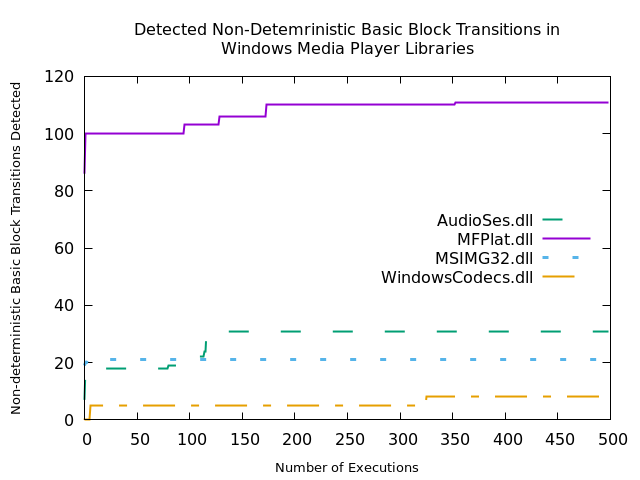
\includegraphics[width=4in]{picker.png}
\caption{Total Non-deterministic Basic Block Transitions Detected per Exeuction}
\label{fig:picker}
\end{figure*}

The algorithm the picker uses is not really compatible will all instrumentation
modules. Anything which uses the \AFL{}-style bitmap will work fine.  This
would include the Dynamo RIO and \AFL{} instrumentation modules. The IPT
instrumentation output is the hashes of the TNT and TIP packets, so any
non-determinism will change every byte of the instrumentation data.  Because of
this, the IPT instrumentation does not have any option to specify the bytes to
ignore, while the DynamoRIO instrumentation does have this.
